

\documentclass[twoside,twocolumn]{article}

\usepackage{blindtext} % Package to generate dummy text throughout this template 
\usepackage{graphicx}
\usepackage[sc]{mathpazo} % Use the Palatino font
\usepackage[T1]{fontenc} % Use 8-bit encoding that has 256 glyphs
\linespread{1.05} % Line spacing - Palatino needs more space between lines
\usepackage{microtype} % Slightly tweak font spacing for aesthetics

\usepackage[english]{babel} % Language hyphenation and typographical rules

\usepackage[hmarginratio=1:1,top=32mm,columnsep=20pt]{geometry} % Document margins
\usepackage[hang, small,labelfont=bf,up,textfont=it,up]{caption} % Custom captions under/above floats in tables or figures
\usepackage{booktabs} % Horizontal rules in tables

\usepackage{lettrine} % The lettrine is the first enlarged letter at the beginning of the text

\usepackage{enumitem} % Customized lists
\setlist[itemize]{noitemsep} % Make itemize lists more compact

\usepackage{abstract} % Allows abstract customization
\renewcommand{\abstractnamefont}{\normalfont\bfseries} % Set the "Abstract" text to bold
\renewcommand{\abstracttextfont}{\normalfont\small\itshape} % Set the abstract itself to small italic text

\usepackage{titlesec} % Allows customization of titles
\renewcommand\thesection{\Roman{section}} % Roman numerals for the sections
\renewcommand\thesubsection{\roman{subsection}} % roman numerals for subsections
\titleformat{\section}[block]{\large\scshape\centering}{\thesection.}{1em}{} % Change the look of the section titles
\titleformat{\subsection}[block]{\large}{\thesubsection.}{1em}{} % Change the look of the section titles

\usepackage{fancyhdr} % Headers and footers
\pagestyle{fancy} % All pages have headers and footers
\fancyhead{} % Blank out the default header
\fancyfoot{} % Blank out the default footer
\fancyhead[C]{DevOps en Base de Datos $\bullet$ Septiembre 2019 $\bullet$ } % Custom header text
\fancyfoot[RO,LE]{\thepage} % Custom footer text

\usepackage{titling} % Customizing the title section

\usepackage{hyperref} % For hyperlinks in the PDF

%----------------------------------------------------------------------------------------
%	TITLE SECTION
%----------------------------------------------------------------------------------------

\setlength{\droptitle}{-4\baselineskip} % Move the title up

\pretitle{\begin{center}\Huge\bfseries} % Article title formatting
\posttitle{\end{center}} % Article title closing formatting
\title{DevOps en Base de Datos} % Article title
\author{Sigfredo Aponte, Alonso Andia, Gabriela Atahuachi y Yhónn Condori}
\date{\today} % Leave empty to omit a date
\renewcommand{\maketitlehookd}{%
\begin{abstract}
\noindent 
This article explains the definition, advantage and the application of DevOps in a Data Base, tools and basic commands for the compression of DevOps and the implementation of this in a database of some application.
\end{abstract}
\begin{abstract}
\noindent 
En el presente artículo se explica la definición, ventajas y la aplicacion de DevOps en una base de datos, ademas de herramientas y porciones de codigo basicas para la comprension general del DevOps y la implementacion de este en una base de datos de alguna aplicacion.
\end{abstract}
}
%----------------------------------------------------------------------------------------
\begin{document}
% Print the title
\maketitle
%----------------------------------------------------------------------------------------
%	ARTICLE CONTENTS
%----------------------------------------------------------------------------------------
\section{Introduccion}
\lettrine[nindent=0em,lines=3]{D}evOps (que equivale a desarrollo y operaciones), al igual que la mayoría de los nuevos enfoques, es solo una expresión de moda que utilizan muchas personas. En un sentido amplio, DevOps es un enfoque basado en principios de agilidad y eficiencia en los que los propietarios de empresas y los departamentos de desarrollo, operaciones y control de calidad colaboran para ofrecer software de forma continua, lo que permite a las empresas sacar partido de las oportunidades del mercado de forma más rápida y reducir el tiempo para incluir respuestas de clientes.
Algunas personas comentan que DevOps solo está destinado a profesionales; otras dicen que gira en torno a la cloud. IBM adopta una visión amplia y holística y considera DevOps como un enfoque de distribución de software orientado a la empresa: un enfoque que adapta una nueva o mejorada capacidad empresarial de llevar una idea durante todo el proceso a producción.[1] 



%------------------------------------------------

\section{Marco Teórico}

\subsection{DevOps}

La mayoría de las descripciones especifican DevOps como un término que se utiliza para enfatizar la colaboración entre el desarrollo de software y las operaciones.

DevOps tiende a resaltar las interacciones entre los individuos y que la tecnología facilita que las interacciones se produzcan fluidamente, eliminando los obstáculos existentes en una organización.[10]

Un objetivo central de DevOps es la automatización y la entrega continua de procesos entre el departamento de operaciones y desarrollo. En otras palabras, DevOps intenta la automatización de tareas repetitivas y tediosas para dejar más tiempo para la interacción humana como valor agregado.[10]

Principios de DevOps:

\begin{itemize}
\item DevOps es un movimiento que cambiar el modo de trabajar en el departamento de tecnología.
\item DevOps intenta solucionar los conflictos entre las áreas desarrollo y operaciones.
\item DevOps se desarrolla dentro de cada empresa.
\item DevOps conforma una retroalimentación efectiva, compartan herramientas, ideas y opiniones.

\end{itemize}


\subsection{Beneficios de DevOps}

El objetivo estratégico general de DevOps es garantizar la calidad del software y satisfacer las necesidades de los clientes. DevOps también permite respuestas rápidas para cambiar los requisitos de los clientes [6]. Con DevOps, los desarrolladores y las operaciones podrían trabajar juntos integrando todos los sistemas organizacionales, simplificando las pruebas y el aseguramiento de la calidad, y suavizando y cerrando la brecha entre el desarrollo y las operaciones [7]. En el entorno DevOps, los errores en el código se corrigen inmediatamente al principio del ciclo de vida del desarrollo de software debido a la implementación continua de compilaciones de software.[5]



%------------------------------------------------

\section{Analisis}

\subsection{Prácticas técnicas para bases de datos}
Las bases de datos tienden a ser un problema particular en DevOps y como en algunos casos para mejorar.
Pero también hay o existen prácticas técnicas que impulsarán su implementación de DevOps con cambios en la base de datos.[3]

\subsection{Migraciones al rescate}
Las migraciones son scripts que incluyen cambios en la base de datos que idealmente son varias pruebas(probar los scripts) para un mismo resultado, lo que significa que no importa cuántas veces ejecute el script, los cambios solo se aplicarán una vez. También es mejor tener los scripts en el control de versiones para que pueda realizar un seguimiento de los cambios y avanzar y retroceder con más facilidad.
En otras palabras, las migraciones son cambios en la base de datos como código. Puede ejecutar exactamente las mismas migraciones en diferentes entornos y los resultados deben ser los mismos, comenzando por el entorno local: la máquina del desarrollador.[3]

\subsection{Practica en un entorno de producción}
Ahora hablaremos de otra práctica técnica que es fácil de implementar pero requiere un poco de disciplina:
las pruebas.
Debe probar un cambio antes de aplicarlo a un entorno de producción. Si los datos de la tabla son enormes, tan grandes que sería costoso replicarlos en un entorno diferente de la producción, asegúrese de que al menos pueda simular el cambio con un conjunto significativo de datos. Esto ayudará a garantizar que el cambio no tome una eternidad y que no bloquee una tabla durante un período prolongado.[3]

\subsection{Herramientas de automatización de bases de datos}
No podemos seguir hablando de bases de datos sin mencionar algunas herramientas. Existen muchas herramientas , y de vez en cuando se lanzan nuevas. Aquí tenemos una lista de las herramientas más populares:
\begin{itemize}
\item Liquibase (gratis)
\item Datical (una versión paga de Liquibase)
\item Redgate (Stack o pila de Microst)
\item Delphix (para cambios u otros fines en la base de datos)
\item DBmaestro (se venden como DevOps para bases de datos)
\end{itemize}

Y además de las herramientas para gestores de bases de datos, también hay marcos que admiten migraciones:

\begin{itemize}
\item Entity Framework
\item GORM
\item Compose
\item Hibernate
\end{itemize}

Como ejemplo, veamos más a fondo Entity Framework en .NET Core.[3]

\subsection{Una guía práctica sobre el uso de Entity Framework Core}
Aunque existen varias herramientas poderosas para automatizar los cambios en la base de datos, echemos un vistazo a un enfoque que puede automatizar fácilmente con herramientas como Jenkins o VSTS utilizando Entity Framework (EF) para aplicaciones .NET Core.
Haremos un cambio simple para que pueda ver cómo EF entra en juego.[3]

\subsection{Configurando su proyecto localmente}
Comencemos abriendo el proyecto con Visual Studio (VS). Deberá tener instalado .NET Core y ejecutará la aplicación con la opción IIS Express. Necesita una instancia de SQL Server para poder instalar / configurar una o utilizar una instalación existente de SQL Server. La idea es que podrá ver cómo se aplican los cambios en la base de datos a medida que avanza.
\begin{center}
	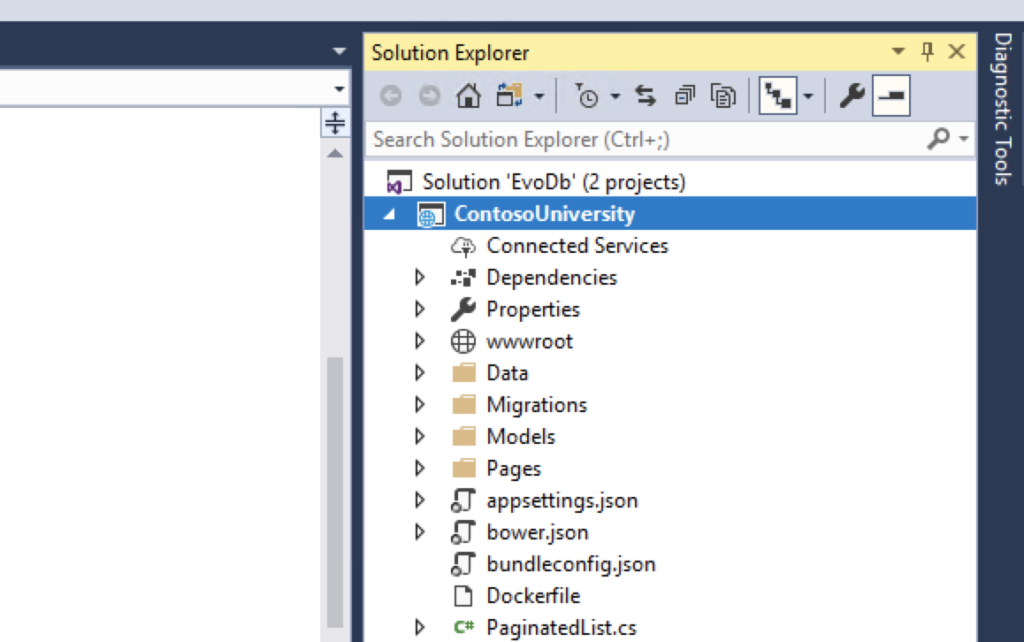
\includegraphics[width=7cm]{./Imagenes/proyecto1} 
	\end{center}
Comencemos cambiando algunos parámetros de entrada para evitar girar la base de datos cuando se inicia la aplicación. Lo haremos manualmente utilizando los comandos de migración de EF. Abra las propiedades del proyecto haciendo clic derecho en el proyecto "ContosoUniversity" y cambie los parámetros de depuración para que se vean así:
\begin{center}
	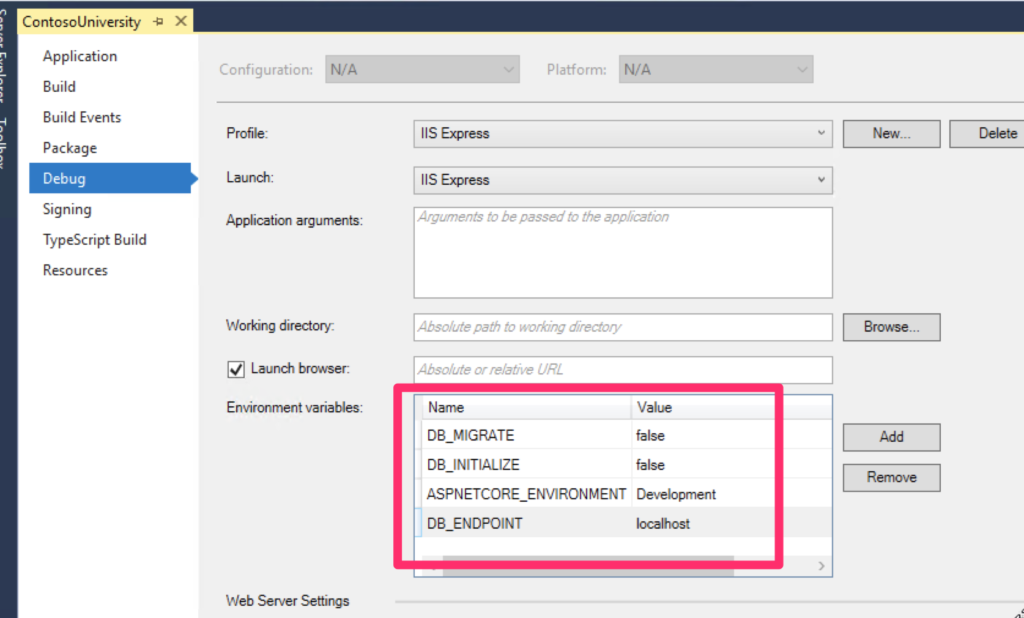
\includegraphics[width=7cm]{./Imagenes/proyecto2} 
	\end{center}
Asegúrese de tener la configuración adecuada para conectarse a la base de datos, especialmente la contraseña de la base de datos. Puede cambiar la contraseña en el archivo appsettings.json . En este caso se tendría que ver algo así(es referencial la foto):
\begin{center}
	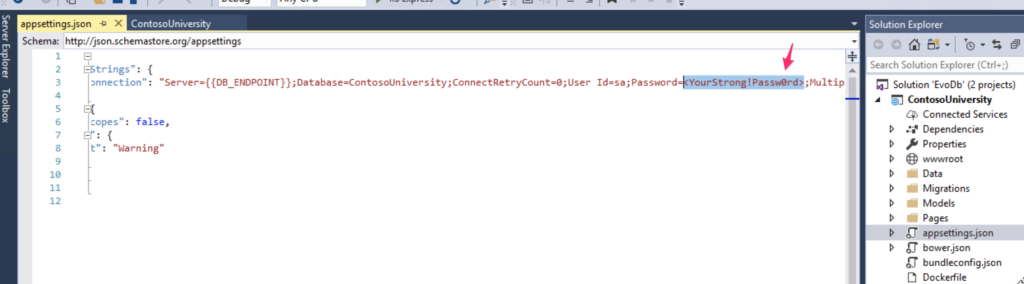
\includegraphics[width=7cm]{./Imagenes/proyecto3} 
	\end{center}
Seleccione el proyecto "ContosoUniversity" y luego ejecútelo haciendo clic en el botón "Depurar". Incluso si la aplicación se inicia, no funcionará porque la base de datos no existe; no hemos ejecutado la primera migración que crea la base de datos.
\begin{center}
	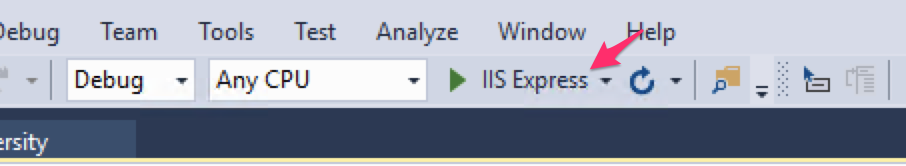
\includegraphics[width=7cm]{./Imagenes/proyecto4} 
	\end{center}

\subsection{Hacer cambios en la aplicación}
Ahora veremos el proceso para hacer cambios en la aplicación añadiendo una nueva columna. Para hacer eso, vamos al archivo Models/Student.cs y añadiremos la columna. Debe quedarnos algo como esto:
\begin{center}
	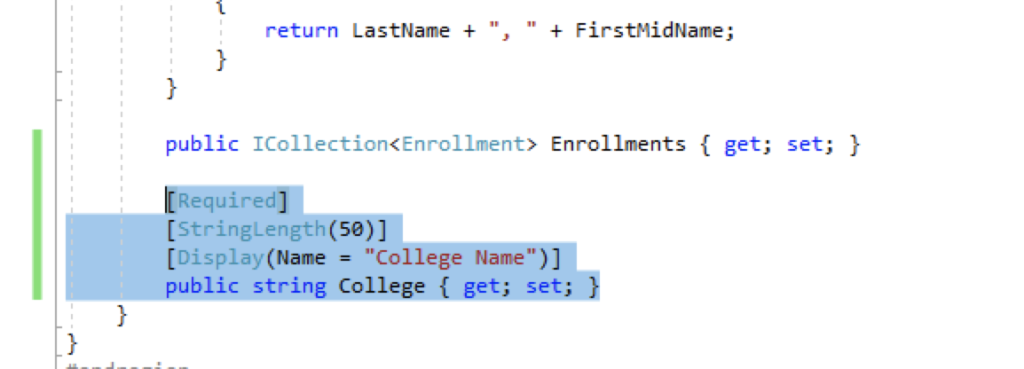
\includegraphics[width=7cm]{./Imagenes/cambios1} 
	\end{center}
Ahora iremos a la vista y añadiremos la columna para ver de una manera mas facil el cambio realizado:
\begin{center}
	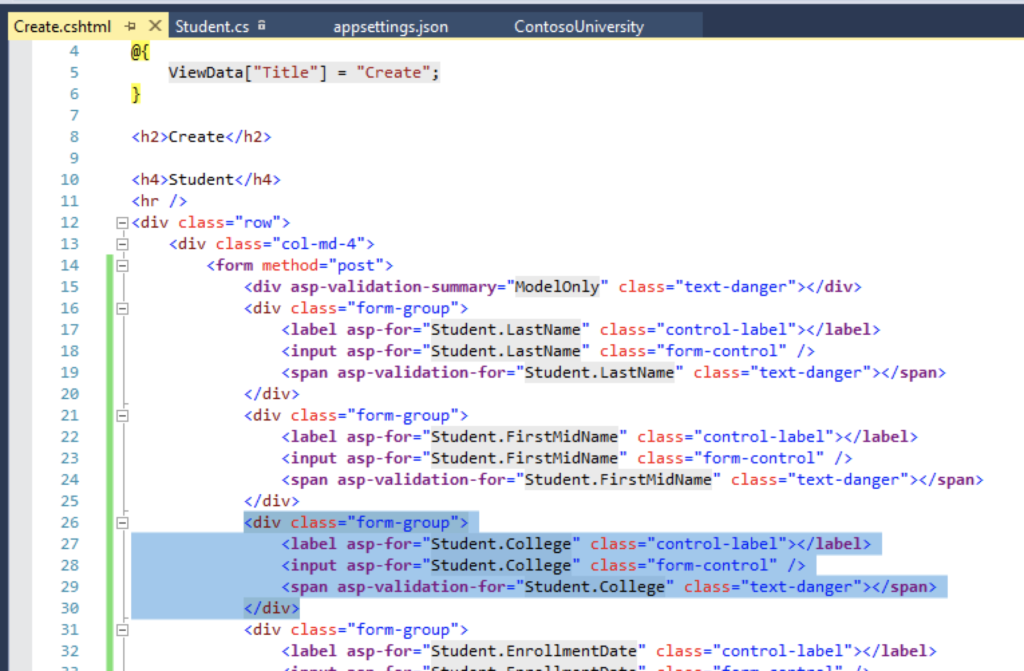
\includegraphics[width=7cm]{./Imagenes/cambios2} 
	\end{center}
Y para persistir la nueva columna, necesitamos cambiar el codigo de la Vista en el archivo Create.cs, como esto:
\begin{center}
	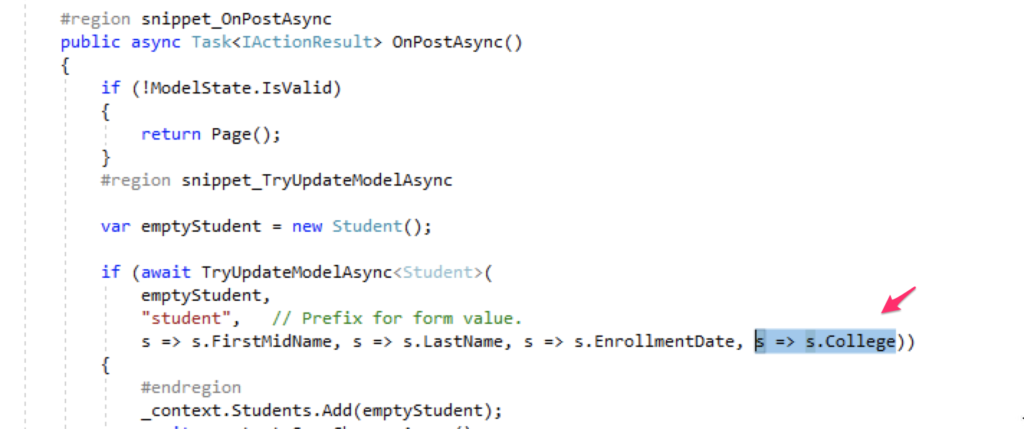
\includegraphics[width=7cm]{./Imagenes/cambios3} 
	\end{center}
Antes de correr la aplicación de nuevo, vamos a crear la migracion en Entity Framework para que la proxima vez que corramos alguna actualizacion en la base de datos, Entity Framework correra cualquier migracion pendiente. Para hacer esto, deberemos ejecutar el comando siguiente:
\begin{center}
	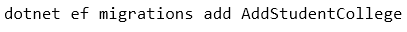
\includegraphics[width=7cm]{./Imagenes/codigo1} 
	\end{center}
Ahora si exploramos la solucion un poco, nos podremos percatar que el nuevo archivo es creado con todos los detalles de la migracion. Y recordando que se necesita tener estos cambios versionados.
\begin{center}
	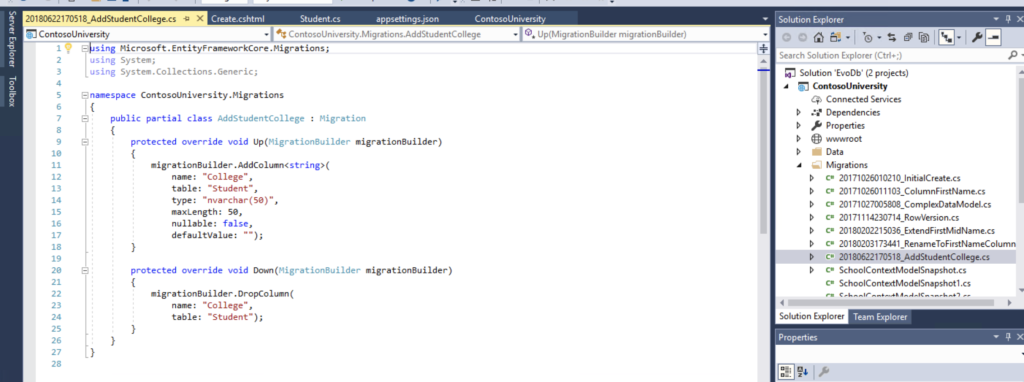
\includegraphics[width=7cm]{./Imagenes/cambios4} 
	\end{center}
Ahora ejecutaremos la aplicación para ver el cambio realizado:
\begin{center}
	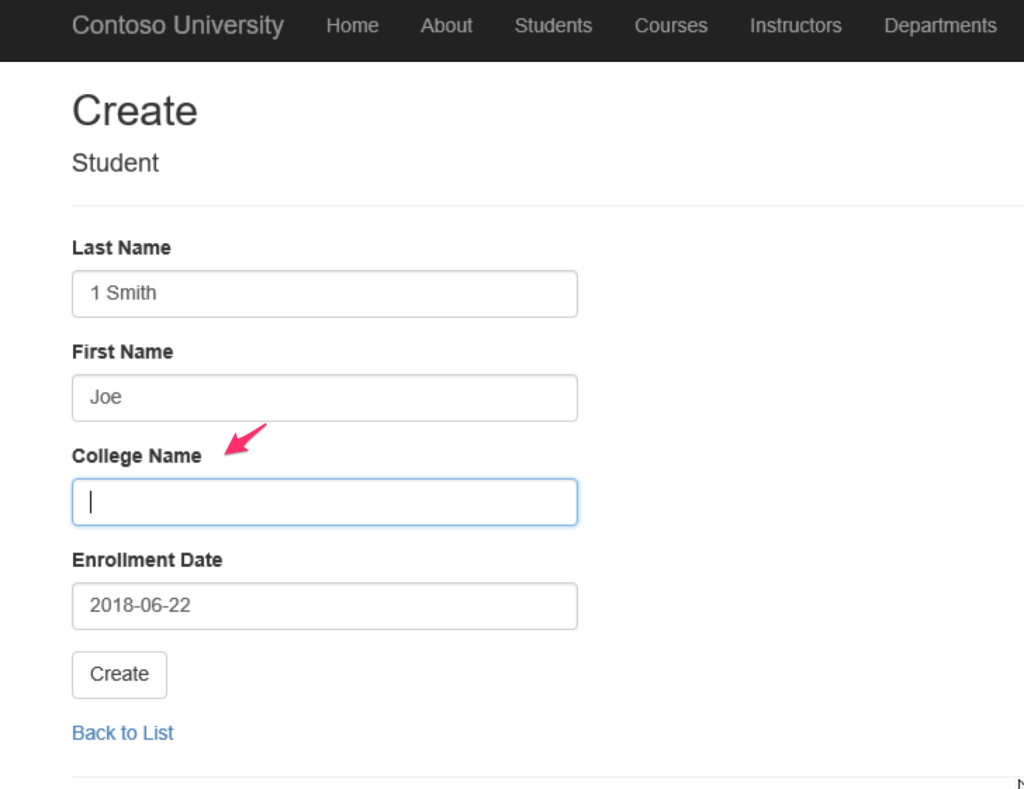
\includegraphics[width=7cm]{./Imagenes/cambios5} 
	\end{center}
La proxima vez que alguien necesite hacer un cambio, una nueva migracion se creara, aplicarlo es solo cuestion de ejecutar el comando de Entity Framework nuevamente. Obviamente conforme mas se valla utilizando, podremos ser mejores en automatizar los cambios de la base de datos. Recordar, que DevOps para base de datos involucra mucho mas que practicas tecnicas. 
\subsection{RollBacks}
Es posible revertir cualquier cambio a la base de datos despues de haber sido actualizada con migraciones recientes. Para hacer eso, solo debemos ejecutar el comando siguiente.
\begin{center}
	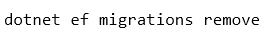
\includegraphics[width=7cm]{./Imagenes/codigo2} 
	\end{center}
Este comando removera la ultima migracion. Eso significa que si mas de una migracion fue aplicada, este comando removera solo la mas reciente. Se necesitara ejecutar el comando mas de una vez si se quiere seguir revirtiendo mas migraciones.

\subsection{Generación de Scripts}
Cuando aun se estan adaptando al proceso, y alguien desea ver exactamente que es lo que el Entity Framework esta hacientdo en la base de datos antes de aplicar cualquier cambio, bueno se puede ver los cambios en formato SQL. Entity Framework tiene un comando para generar scripts en formato SQL que cualquier Administrado de Base de datos puede enterner.
Para generar las migraciones en formato SQL, ejecutaremos el siguiente comando:
 \begin{center}
	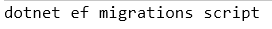
\includegraphics[width=7cm]{./Imagenes/codigo3} 
	\end{center}
Todas las declaraciones de SQL que necesitas apareceran en el terminal. Puedes guardar la salida de codigo en un archivo para revisarlo despues.
 \begin{center}
	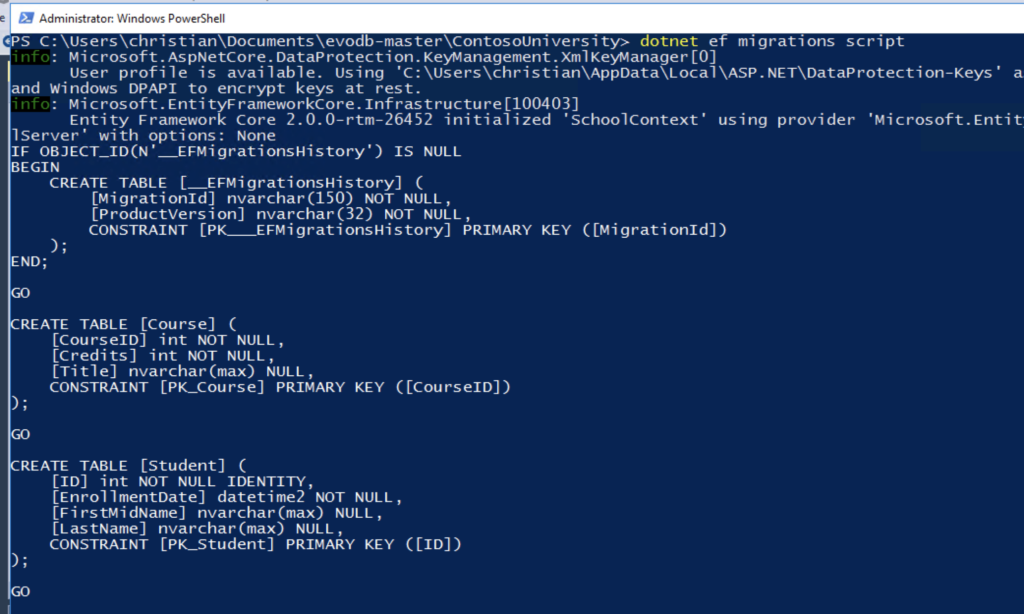
\includegraphics[width=7cm]{./Imagenes/scripts} 
	\end{center}
Como se puede ver no existe una formula para la implementacion de DevOps en Bases de datos, existen muchas cosas que estan involucradas, pero el primer paso es salir de la zona de confort y hacer las cosas mejor. Debemos ir implementando cambios, que a veces provocan temor, especialmente cuando hablamos de datos, pero se debe intentar mantener las cosas lo mas simples posibles, desde los procesos a la arquitectura.Se debe enfocar en tener una arquitectura que nos permita realizar cambios sin muchas molestias, e ir estudiando las diferentes posibildades de automatizacion que nos dan las diferentes herramientas de trabajo que tenemos. Los cambios en una base de datos no suelen ser tan dificiles como aparentan, el problema son las potenciales perdidas o daños de toda o una porcion de los datos, la repeticion y constancia son la clave, para saber que hacer y que no. [3]



\section{Conclusiones}
\begin{itemize}
\item DevOps depende de la comunicación, pero una mejor comunicación asociada a procesos ineficientes no se traduce en mejores implementaciones.
\item DevOps no está destinado a sistemas grandes y complejos.[6]
\item DevOps no está destinado al desarrollo externalizado.
\item Si algo caracteriza a DevOps es la automatización.
\item Algunos gurús lo definen como metodología, otros como una cultura estrechamente ligada a entornos ágiles.[7]

\end{itemize}

%	REFERENCE LIST
%----------------------------------------------------------------------------------------

\begin{thebibliography}{99} % Bibliography - this is intentionally simple in this template
\bibitem[1]{Sanjeev Sharma:2014dg}
Sanjeev Sharma (2014).
\newblock DevOps para Dummies

\bibitem[2]{Elena Sanchez:2019dg}
Elena Sanchez (2019).
\newblock Introducción a DevOps. Qué es y cómo implementarlo

\bibitem[3]{Christian Melendez:2018dg}
Christian Melendez (2018).
\newblock DevOps for Databases

\bibitem[4 ]{Michael Hüttermann:2012dg}
Michael Hüttermann (2012).
\newblock DevOps for Developers

\bibitem[5]{Research and Markets :2015dg}
Research and Markets (2015).
\newblock Research and Markets: Global DevOps Tool Market to Grow at a CAGR of 14.97 percent  over the Period 2014-2019

\bibitem[6]{J. Wettinger, U. Breitenbücher, and F. Leymann :2014dg}
J. Wettinger, U. Breitenbücher, and F. Leymann (2014).
\newblock DevOpSlang–bridging the gap between development and operations

\bibitem[7]{J. Smeds, K. Nybom, and I. Porres :2015dg}
J. Smeds, K. Nybom, and I. Porres (2015).
\newblock DevOps: A Definition and Perceived Adoption Impediments

\bibitem[8]{Mike Lookides :2012dg}
Mike Lookide (2012).
\newblock What is DevOps?

\bibitem[9]{Julio Sandobalín-Guamán,  Miguel Zúñiga-Prieto,  Emilio Insfran, Silvia Abrahão, Carlos Cano  :2014dg}
Julio Sandobalín-Guamán,  Miguel Zúñiga-Prieto,  Emilio Insfran, Silvia Abrahão, Carlos Cano (2014).
\newblock Una aproximación DevOps para el Desarrollo Dirigido por Modelos de Servicios Cloud 

\bibitem[10]{Fernando Becerra :2018dg}
Fernando Becerra (2018).
\newblock Implementación de una Solución para el problema Shared Bottleneck del Protocolo MP-TCP Utilizando SDN Sobre una Infraestructura de Computación en la Nube
 
\end{thebibliography}

%----------------------------------------------------------------------------------------

\end{document}
